\documentclass[12pt]{article}
\usepackage[utf8]{inputenc}
\usepackage[T2A]{fontenc}
\usepackage[russian]{babel}
\usepackage{amsmath}
\usepackage{amssymb}
\usepackage{dsfont}
\usepackage[dvipsnames]{xcolor}
\usepackage{setspace}
\usepackage{multirow}
\usepackage[a4paper, outer=1.5cm, inner=1.5cm, top=1cm, bottom=1cm]{geometry}
\usepackage{graphicx}
\usepackage{skull}
\usepackage{wasysym}
\usepackage{float}
\graphicspath{{.images/}}
\usepackage{hyperref}
\hypersetup{colorlinks=true, linkcolor=blue, filecolor=magenta, urlcolor=cyan}
\usepackage[firstpage]{draftwatermark}
\SetWatermarkText{
    $\qquad\qquad\qquad\qquad\qquad$\parbox{7cm}{\begin{center}
    
\includegraphics[width = 0.08\textwidth]{lion-logo.png}\bigskip\\~\bigskip\\~\vspace{-24mm}\\~\end{center}}
}
\SetWatermarkAngle{0}
\SetWatermarkScale{1.5}
\usepackage{etoolbox}

\newtoggle{ifsolved}
\newtoggle{needhelp}
\newcounter{num}
\setcounter{num}{1}

\newcommand{\newnum}{\par\textbf{\textnumero\arabic{num}}\stepcounter{num}}
\newcommand{\sol}{\vspace{3mm}\par\textbf{Решение: }}
\newcommand{\ans}{\vspace{3mm}\par\textbf{Ответ: }}
\newcommand{\hint}{\vspace{3mm}\par\textbf{Подсказка: }}
\newcommand{\mode}[1]{
\ifstrequal{#1}{0}{\togglefalse{ifsolved}\togglefalse{needhelp}}{\ifstrequal{#1}{1}{\togglefalse{ifsolved}\toggletrue{needhelp}}{\ifstrequal{#1}{2}{\toggletrue{ifsolved}\togglefalse{needhelp}}{\toggletrue{ifsolved}\toggletrue{needhelp}}}}} %if 0 - if 1 - if 2 - else
%\newenvironment{problem}[8]{%#1, #2, #3
%\parbox{\linewidth}{\vspace{4mm}\ifstrequal{#4}{(лёгкая)}{\newnum\textbf{.}}{\newnum\textbf{*.} } \\ #5}
%\iftoggle{ifsolved}{\sol #6}{}
%\iftoggle{ifsolved}{\ans #7}{}
%\iftoggle{needhelp}{\hint #8}{}}

\newenvironment{problem}[8]{%#1, #2, #3
\parbox{\linewidth}{\vspace{5mm}\ifstrequal{#4}{(лёгкая)}{\newnum\textbf{.}}{\newnum\textbf{*.} } \\ #5}
\iftoggle{ifsolved}{\sol #6}{}

\iftoggle{ifsolved}{\parbox{\linewidth}{\ans #7}}{}
\iftoggle{needhelp}{\parbox{\linewidth}{\hint #8}}{}}

\newenvironment{mylist} %custom list
{ \begin{itemize}
    \setlength{\itemsep}{0pt}
    \setlength{\parskip}{0pt}
    \setlength{\parsep}{0pt}     }
{ \end{itemize}                  }

\newenvironment{homeass}[1]{\vspace*{-1.5cm}
\iftoggle{ifsolved}{
    \section*{\center{Решение домашнего задания к #1.}}
}{
    \section*{\center{\textcolor{Sepia}{Домашнее задание к #1}}}
} \vspace{7mm}\large}

\parindent=0pt
\pagestyle{empty}
%$\!$[\arabic{class}.\arabic{num}]
%\ifnumcomp{\value{counter}}{>}{1}{true}{false}
%\definecolor{Gray}{gray}{0.9}
%\definecolor{mypink}{RGB}{219, 48, 122}
%\newcolumntype{g}{>{\columncolor{Gray}}p{2.8cm}}

\begin{document}
\large
\mode{7}
%0 for problems without hints
%1 for problems + hints
%2 for problems + solutions + answers
%else: show all

{\centering\section*{СПИСОК ЗАДАЧ}}

{\centering\subsection*{\smallskip\\\textcolor{green}{\textbf{Полезные вещи, которые можно и нужно копипастить:}}}}

\subsection*{\textcolor{Emerald}{\textbf{Полезные шпаргалки по LaTeXу:}}}

\textbf{Пример вставки рисунка:}

\begin{minipage}{\linewidth}
    \begin{minipage}{0.54\linewidth}
    см. рисунок справа\\
    Текст к собственно пикче, примерно всегда это либо развёрнутое описание, либо большая часть решения задачи --- стремимся экономить пространство, если это можно сделать.
    \end{minipage}
    \hspace{0.05\linewidth}
    \begin{minipage}{0.4\linewidth}
    \begin{figure}[H] 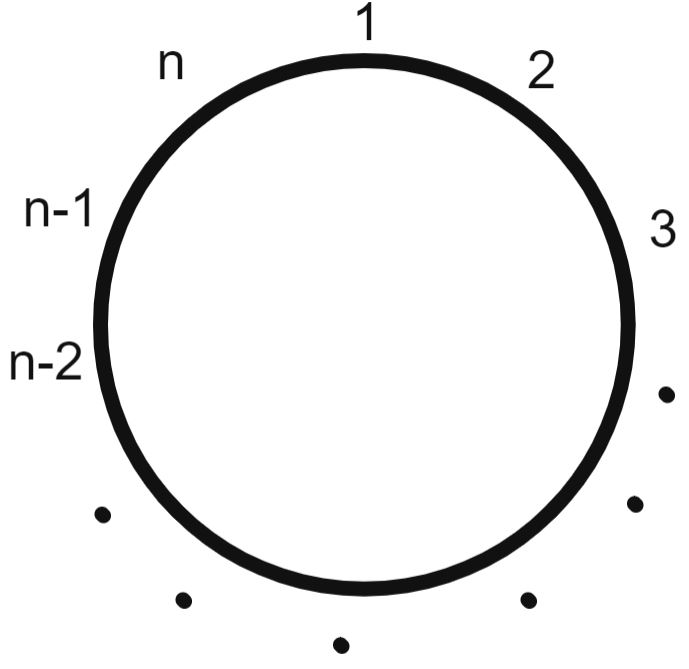
\includegraphics[width=\linewidth]{sol3} %тут поменять имя пикчи
    \end{figure}
    \end{minipage}
\end{minipage}

\textbf{Дефолтные математические знаки и символы:}\\
$\geqslant$,
$\leqslant$,
$a^{b}$,
$x_{i}$,
$\sqrt{a}$,
$\frac{a}{b}$,
$\displaystyle \frac{a}{b}$,
$\cdot$
$\;\Rightarrow\;$,
$\;\Leftrightarrow\;$,
$1{,}2$.
О промежутках:
$a\!b$,
$a\,b$,
$a\:b$,
$a\;b$,
$a\quad b$.

\textbf{Стандартные система и совокупность уравнений / неравенств:}\\
$\left\{
\begin{aligned}
f(x) &= 0 \\
g(x) &= 1
\end{aligned}\right.$

$\left[\begin{aligned}
&\left\{\begin{aligned}
f(x) &\geqslant a \\
g(x) &= b
\end{aligned}\right.\\
&\left\{\begin{aligned}
f(x) &< a \\
g(x) &= -b
\end{aligned}\right.
\end{aligned}\right.$

\subsection*{\textcolor{Emerald}{\textbf{Не математическое, но полезное:}}}
% комментарий в любом месте документа, который нигде не будет видно. Можно использовать для написания заметок-вопросов по задачам
\textbf{Пример таблицы:}

\begin{tabular}{|c|c|c|}
\hline
    $a$ & $b$ & текст
\\\hline
    $c$ & $d$ & мораль
\\\hline
\end{tabular}\\

\textbf{Отступы:} между\smallskip\\ строками\medskip\\ \textbf{Тире} --- это три дефиса.\\
\textbf{Списки:}
\begin{mylist}
\item [$\bullet$] это был пункт а
\item [2)] а это уже пункт номер 2 с изменённым заголовком
\end{mylist}

\subsection*{\textcolor{Emerald}{\textbf{Всё, неупомянутое выше (или если просто что-то не так):}}}
\begin{mylist}
\item [$\bullet$] Решение отдельных вопросов касательно ТеХа нужно искать в \href{https://www.mccme.ru/free-books/llang/newllang.pdf}{Львовском}.

\item [$\bullet$] Найти произвольный символ, который нужен, можно в \href{http://detexify.kirelabs.org/classify.html}{Detexify}.

\item [$\bullet$] Если возникли сомнения при решении, ответ практически ко всем задачам можно проверить с помощью \href{https://www.wolframalpha.com/}{WolframAlpha}.

\item [$\bullet$] Если в задаче нужно создать картинку, то лучше пока отложить эту задачу. Все графики планируется централизованно нарисовать (или перерисовать) в геогебре.

\item [\textcolor{brown}{\textbf{!!}}] Важно ставить \textcolor{red}{\textbf{$\spadesuit$}}
(или просто red) в тело задачи в случае серьёзных вопросов к решению и какой-то вопиющей лажи.

\item [\textcolor{brown}{\textbf{!!}}] Важно ставить \textcolor{olive}{\textbf{$\spadesuit$}}
(или просто olive) в тело задачи в случае не самого удачного текста и кривых отступов.
\end{mylist}

\subsection*{\textcolor{Violet}{\textbf{Комментарии:}}}% а также невидимые комментарии - так можно оставлять заметки-вопросы прямо в задаче, чтобы потом было понятно, в чём вопрос.
\begin{mylist}
\item [$\skull$] Переставлять задачи местами --- очень плохая идея.

\item [$\smiley$] При двойном клике по тексту pdf справа происходит автоматический переход к этому месту в латех-коде, а для обратного перехода можно нажать стрелку вправо (висит сверху между pdf и латех-кодом).

\item [$\smiley$] Если есть размышления, дописывать red/olive к задаче или не дописывать, то лучше всё-таки дописать.

\item [$\skull$] Самое плохое, что можно сделать --- написать в любое поле из трёх (НаписанноеРешение/ВерныйОтвет/Подсказка) только половину того, что надо, никак это не отметить, и потом пойти дальше.\\ Нужно в этот момент писать red/olive в случайном месте задачи, чтобы потом вычислить это с помощью Ctrl+F по всему документу (и это то, что потом будет делаться долго и тщательно)
\end{mylist}

\newpage
\setcounter{num}{35}

\hypertarget{6.2}{{\centering\section*{\bigskip\\\textcolor{Blue}{\hyperlink{start2}{\textcolor{Blue}{6.2}} Сложение и вычитание дробей.}\vspace{-5mm}}}}

\begin{problem}{Основное свойство дроби.}{6.2.1}{6S}{(лёгкая)}
{При каких натуральных значениях $m$ дробь $\displaystyle\frac{6}{m + 1}$ будет неправильной?}
{По определению, неправильная дробь~--- такая, у которой числитель больше чем знаменатель или равен ему. То есть $6 \geqslant m + 1$. Это означает, что при $m = 6$ дробь не будет неправильной, а будет при $m \leqslant 5$. Следовательно, подходят значения $m = 1$, $m = 2$, $m = 3$, $m = 4$, $m = 5$ (получаются дроби $\frac62$, $\frac63$, $\frac64$, $\frac65$, $\frac66$, которые все являются неправильными).}
{Дробь будет неправильной при $m = 1$, $m = 2$, $m = 3$, $m = 4$, $m = 5$.}{У неправильной дроби числитель...}
\end{problem}

\begin{problem}{Основное свойство дроби.}{6.2.1}{6S}{*}
{При каких натуральных значениях $k$ дробь $\displaystyle\frac{k - 4}{11}$ будет правильной?}
{НаписанноеРешение}
{ВерныйОтвет}{Подсказка}
\end{problem}

\begin{problem}{Основное свойство дроби.}{6.2.1}{6S}{*}
{Известно, что дробь $\displaystyle\frac{\text{В} \cdot \text{А} \cdot \text{Р} \cdot \text{Е} \cdot \text{Н} \cdot \text{Ь} \cdot \text{Е}}{\text{К} \cdot \text{А} \cdot \text{Р} \cdot \text{Л} \cdot \text{С} \cdot \text{О} \cdot \text{Н}}$~--- целое число, где разные буквы обозначают разные цифры, а между ними стоит знак умножения. Чему равна дробь?}
{В данном примере-ребусе очень много различных букв, а именно 10 штук: $\text{В}$ $\text{А}$, $\text{Р}$, $\text{Е}$, $\text{Н}$, $\text{Ь}$, $\text{К}$, $\text{Л}$, $\text{С}$, $\text{О}$. Но поскольку различных цифр всего 10 (0-9), и каждая буква обозначает свою цифру, какая-то из этих цифр равна нулю!\\
Подумаем о том, где же этот ноль находится. Делить на ноль, как мы знаем, нельзя (тогда у нас целого числа уж точно не получится)~--- поэтому в <<слове>> КАРЛСОН его нет. Это значит, что 0 стоит в числителе. Тогда независимо от других цифр, числитель этой дроби будет равен нулю и сама дробь равна 0. }
{Дробь равна 0. Пример ответа: $\,\displaystyle\frac{0 \cdot 9 \cdot 8 \cdot 7 \cdot 6 \cdot 5 \cdot 7}{4 \cdot 9 \cdot 8 \cdot 3 \cdot 2 \cdot 1 \cdot 6} = \frac{0\cdot 5\cdot 49}{24} = \frac{0}{24} = 0$.}{Сколько всего различных цифр в этом примере?}
\end{problem}

\begin{problem}{Приведение дробей к общему знаменателю.}{6.2.3}{6S}{(лёгкая)}
{В классе учится меньше, чем 50 человек. За контрольную работу $\frac{1}{7}$ учеников получили пятёрки, $\frac{1}{3}$~--- четвёрки, $\frac{1}{2}$~--- тройки. Все остальные работы были оценены на <<2>>. Сколько было таких работ?}
{НаписанноеРешение}
{ВерныйОтвет}{Подсказка}
\end{problem}

\begin{problem}{Приведение дробей к общему знаменателю.}{6.2.3}{6S}{*}
{Сначала отпили $\frac{1}{6}$ чашки чёрного кофе и долили молока. Потом выпили $\frac{1}{3}$ чашки и снова долили молока. Потом выпили ещё полчашки и снова долили молока. Наконец, выпили полную чашку.\\ Чего в итоге выпили больше~--- кофе или молока?}
{НаписанноеРешение}
{ВерныйОтвет}{Подсказка}
\end{problem}

\begin{problem}{Сравнение, сложение и вычитание дробей.}{6.2.4}{56 red переместительный для вычитания?}{(лёгкая)}
{Решить уравнение: $\;\displaystyle \left(x - \frac{1}{4}\right) + 3\frac{1}{12} = 7\frac{1}{3}$}
{НаписанноеРешение}
{ВерныйОтвет}{Подсказка}
\end{problem}

\begin{problem}{Сравнение, сложение и вычитание дробей.}{6.2.4}{56}{(лёгкая)}
{Сравнить числа, выполнив необходимые действия: $\;0{,}65$ и $\frac{13}{25}$.}
{Первый способ (одинаковые знаменатели): $\frac{13}{25} = \frac{52}{100} = 0{,}52$.\\ $0{,}65 > 0{,}52$, следовательно, первое число больше.\\
Второй способ (одинаковые числители): $0{,}65 = \frac{65}{100} = \frac{13}{20}$. Числители двух дробей равны, но знаменатель первой дроби меньше, следовательно, первое число больше.}
{$0{,}65 > \frac{13}{25}$, первое число больше.}{Сравнивать можно как две дроби с равными знаменателями, так и две дроби с равными числителями. В этой задаче можно выбрать любой способ.}
\end{problem}

\begin{problem}{Сравнение, сложение и вычитание дробей.}{6.2.4}{6S}{(лёгкая)}
{Найди дробь, которая больше одной из данных дробей, но меньше другой: $\displaystyle\frac{3}{7}$, $\displaystyle\frac{2}{9}$.}
{Отметим, что дробь $\displaystyle\frac ab$, которую мы ищем, больше $\displaystyle\frac{2}{9}$ и меньше $\displaystyle\frac{3}{7}$, то есть $\displaystyle\frac{2}{9} < \frac ab < \frac{3}{7}$.\\ Универсальное решение тут следующее: приведём дроби к общему знаменателю (в этом случае это НОК(9, 7) $=$ 63). Тогда $\frac29 = \frac{2 \cdot 7}{9 \cdot 7} = \frac{14}{63}$, $\,\frac37 = \frac{3 \cdot 9}{7 \cdot 9} = \frac{27}{63}$, и $\frac{14}{63} < \frac ab < \frac{27}{63}$.\\ Довольно очевидно, что если взять $b = 63$ (такой же знаменатель), а число $a$ находится между 15 и 26 $(15 \leqslant a \leqslant 26)$, то такая дробь подойдёт под условие задачи. Например, при $a = 21$ получается дробь $\,\frac{21}{63} = \frac39 = \frac13$, и $\,\frac29 < \frac13 < \frac 37$\\ (хотя есть и другие варианты, у которых знаменатели никак не связаны с 63).}
{Под условие подходит множество дробей, например, $\frac13$.}{Какая дробь больше, а какая меньше?}
\end{problem}

\begin{problem}{Сравнение, сложение и вычитание дробей.}{6.2.4}{6S}{*}
{Приведи пример дроби, знаменатель которой меньше 10, и которая при этом больше $\frac{7}{9}$, но меньше $\frac{8}{9}$.}
{Понятно, что знаменатель этой дроби~--- не 9. Значит, есть восемь вариантов (знаменатель гипотетически может быть любым натуральным числом от 1 до 8). Дроби $\frac79$ и $\frac89$ близки к единице, но всё же чуть меньше её. \\
Проверим все варианты: $\frac11$ не подходит (и вообще надо получить меньше единицы), $\frac12$ не подходит ($\frac12 = \frac{9}{18} < \frac{14}{18} = \frac79$), $\frac23$ не подходит ($\frac23 = \frac69 < \frac79$), $\frac34$ не подходит ($\frac34 = \frac{27}{36} < \frac{28}{36} = \frac79$). Осталось 4 варианта~--- дроби со знаменателями 5, 6, 7, 8.\smallskip\\ Проверяем: $\frac45$ подходит ($\frac45 = \frac{36}{45} > \frac{35}{45} = \frac79$), понятно, что она меньше $\frac89 = \frac{40}{45}$.\smallskip\\
$\frac56$ подходит ($\frac56 = \frac{45}{54} > \frac{42}{54} = \frac79$), она также меньше $\frac89 = \frac{48}{54}$.\smallskip\\
$\frac67$ подходит ($\frac67 = \frac{54}{63} > \frac{49}{63} = \frac79$), она всё ещё меньше $\frac89 = \frac{56}{63}$.\smallskip\\
Наконец, $\frac78$ тоже подходит ($\frac78 = \frac{63}{72} > \frac{56}{63} = \frac79,\,$ и $\,\frac89 = \frac{64}{72}$).}
{Таких дробей четыре: это дроби $\frac45$, $\frac56$, $\frac67$, $\frac78$. Других нет.}{Знаменатель этой дроби~--- не 9.}
\end{problem}

\begin{problem}{Сравнение, сложение и вычитание дробей.}{6.2.4}{6S}{*}
{Сравни дроби: $\displaystyle\frac{12}{35}$ и $\displaystyle\frac{72}{211}$;
$\quad\displaystyle\frac{22}{35}$ и $\displaystyle\frac{110}{177}$; $\quad\displaystyle\frac{1998}{1999}$ и $\displaystyle\frac{1999}{2000}$.}
{НаписанноеРешение}
{ВерныйОтвет}{Подсказка}
\end{problem}

\begin{problem}{Сравнение, сложение и вычитание дробей.}{6.2.4}{56}{*}
{Сравнить числа, использовав хитрость: $\;\displaystyle\frac{3025}{3026}\,$ и $\,\displaystyle\frac{5035}{5036}$}
{Отметим, что оба числа весьма незначительно отличаются от единицы. Первое число отличается от 1 на $\frac{1}{3026}$, второе~--- на $\frac{1}{5036}$. Поскольку дроби $\frac{1}{3026}$ и $\frac{1}{5036}$ имеют одинаковые числители, мы можем их сравнить: $3026 < 5036$, а значит $\frac{1}{3026} > \frac{1}{5036}$ (из двух дробей с одинаковыми числителями больше та, у которой знаменатель меньше). Тогда получается, что вначале эти числа были оба равны 1, а потом из них вычли разные дроби. Поскольку $\frac{1}{3026} > \frac{1}{5036}$, в первом случае было вычтено большее число. Значит, в итоге результат в первом случае получится меньше, то есть $\frac{3025}{3026} < \frac{5035}{5036}$ (второе число ближе к единице).}
{$\frac{3025}{3026} < \frac{5035}{5036}$, вторая дробь больше.}{Оба числа не сильно отличаются от 1... А каково это отличие?}
\end{problem}

\begin{problem}{Сравнение, сложение и вычитание дробей.}{6.2.4}{6S}{*}
{Представь $1\frac{1}{12}$ в виде суммы трёх дробей, числители которых равны 1.}
{Перепишем условие задачи: $1\frac{1}{12} = \frac{13}{12} = \frac1? + \frac1? + \frac1?$. Это означает, что 12~--- НОК этих трёх знаменателей. Если знаменатель какой-то дроби равен 12, то получается один возможный вариант $\frac1{12} + \frac12 + \frac12$. Если такой дроби нет, то есть ещё один вариант, если знаменатели равны 2, 3, 4: $\frac12 + \frac13 + \frac14 = \frac{6}{12} + \frac{4}{12} + \frac{3}{12} = \frac{6 + 4 + 3}{12} = 1\frac{1}{12}$.}
{$1\frac{1}{12} = \frac1{12} + \frac12 + \frac12\,$ или $\,1\frac{1}{12} = \frac12 + \frac13 + \frac14$.\\
\textbf{Комментарий:} Чтобы заметить более хитрый способ решения, можно выписать подряд делители числа 12 и выбрать те, что дают в сумме 13: $\,$1, 2, \textcolor{orange}{\underline{\underline{3}}}, \textcolor{orange}{\underline{\underline{4}}}, \textcolor{orange}{\underline{\underline{6}}}, 12.}{Может быть полезно взглянуть на круглый циферблат часов.}
\end{problem}

\begin{problem}{Сравнение, сложение и вычитание дробей.}{6.2.4}{6S}{*}
{Докажи, что значение суммы $\frac{1}{1001} + \frac{1}{1002} + \ldots + \frac{1}{2000}$ больше, чем $\frac{1}{2}$.}
{На самом деле, для решения задачи надо просто описать, что нужно посчитать. Сумма состоит из 1000 слагаемых, от $\frac{1}{1001}$ до $\frac{1}{2000}$.\\ Было бы гораздо проще посчитать эту сумму, если бы знаменатели были одинаковыми: например $\frac{1}{1000} + \frac{1}{1000} + \ldots + \frac{1}{1000} = 1\,$ и $\,\frac{1}{2000} + \frac{1}{2000} + \ldots + \frac{1}{2000} = \frac{1000}{2000} = \frac12$.\smallskip\\ Нам как раз и надо показать, что наша сумма больше, чем $\frac12$. Почему так?\smallskip\\ Интуитивно понятно, что наша сумма~--- нечто между $\frac12$ и 1. Строго говоря, любая дробь в нашем выражении, кроме последней, строго больше $\frac{1}{2000}$: из двух дробей с одинаковыми числителями больше та, знаменатель которой меньше.\\ А если каждая дробь в нашей сумме больше чем $\frac{1}{2000}$, то при замене каждой дроби на $\frac{1}{2000}$ получится меньшее значение (равное $\frac12$). Доказано!}
{Смотри рассуждение выше.}{Сколько здесь всего слагаемых?\\ Какую дробь надо выбрать, чтобы взяв её столько раз, мы бы получили $\frac12$?\\ Как наше выражение отличается от этого примера?}
\end{problem}

\begin{problem}{Сравнение, сложение и вычитание дробей.}{6.2.4}{6S}{*}
{Можно ли число 1 представить в виде $\frac{1}{a} + \frac{1}{b} + \frac{1}{c} + \frac{1}{d}$, где $a$, $b$, $c$, $d$~--- нечётные натуральные числа?}
{НаписанноеРешение}
{ВерныйОтвет}{Подсказка}
\end{problem}

\begin{problem}{Сравнение, сложение и вычитание дробей.}{6.2.4}{6S}{(лёгкая)}
{Найди число, которое на столько же меньше $5\frac{5}{12}$, на сколько $3\frac{5}{9}$ меньше $6\frac{1}{3}$.}
{НаписанноеРешение}
{ВерныйОтвет}{Подсказка}
\end{problem}

\begin{problem}{Сравнение, сложение и вычитание дробей.}{6.2.4}{6S}{(лёгкая)}
{Найди число, которое на столько же больше $4\frac{9}{12}$, на сколько $4\frac{8}{9}$ меньше $7\frac{1}{4}$.}
{На сколько $4\frac{8}{9}$ меньше $7\frac{1}{4}$? Найдём разность: $7\frac{1}{4} - 4\frac{8}{9} = 7\frac{9}{36} - 4\frac{32}{36} = 2\frac{13}{36}$.\smallskip\\
Число больше $4\frac{9}{12}$ на $2\frac{13}{36}$, а значит равно $4\frac{9}{12} + 2\frac{13}{36} = 4\frac{27}{36} + 2\frac{13}{36} = 6 + \frac{40}{36} = 7\frac{4}{36} = 7\frac19$.}
{Искомое число равно $7\frac19$.}{Вычисли, на сколько $4\frac{8}{9}$ меньше $7\frac{1}{4}$.}
\end{problem}

\begin{problem}{Сравнение, сложение и вычитание дробей.}{6.2.4}{6S}{(лёгкая)}
{Допиши равенства: $\;\displaystyle\vphantom{\rule{0pt}{18pt}}\frac{1}{2 \cdot 3} = \frac{1}{2} - \frac{1}{3};\qquad \frac{1}{3 \cdot 4} = \frac{1}{3} - \frac{1}{?};\qquad \frac{1}{4 \cdot 5} = \frac{1}{?} - \frac{1}{?}$\smallskip\\
Используя эту закономерность, найди сумму:  $\;\displaystyle\vphantom{\rule{0pt}{18pt}}\frac{1}{1 \cdot 2} + \frac{1}{2 \cdot 3} + \frac{1}{3 \cdot 4} + \frac{1}{4 \cdot 5} + \frac{1}{5 \cdot 6} = {?}$

}
{Проверим первое равенство: $\frac{1}{2} - \frac{1}{3} = \frac{3}{2\cdot3} - \frac{2}{2\cdot 3} = \frac{3 - 2}{2\cdot3} = \frac{1}{2\cdot3}$.\\ То есть знаменатель получается произведением знаменателей (потому что два идущих подряд числа можно только перемножить, НОК($n, n\!+\!1$) $= n(n+1)$), а сверху получается единица, потому что разница двух соседних чисел равна 1.\\ Поэтому $\frac{1}{3 \cdot 4} = \frac{4}{3\cdot4} - \frac{3}{3\cdot 4} = \frac{1}{3} - \frac{1}{4}$ и $\frac{1}{4 \cdot 5} = \frac{5}{4\cdot5} - \frac{4}{4\cdot 5} = \frac{1}{4} - \frac{1}{5}$. Тогда, если это использовать,
$\displaystyle\vphantom{\rule{0pt}{18pt}}\frac{1}{1 \cdot 2} + \frac{1}{2 \cdot 3} + \frac{1}{3 \cdot 4} + \frac{1}{4 \cdot 5} + \frac{1}{5 \cdot 6} = \left(\frac11 - \frac12\right) + \left(\frac12 - \frac13\right) + \left(\frac13 - \frac14\right) + \left(\frac14 - \frac15\right) + \left(\frac15 - \frac16\right) = \frac11 - \frac12 + \frac12 - \frac13 + \frac13 - \frac14 + \frac14 - \frac15 + \frac15 - \frac16 = 1 - \frac16 = \vphantom{\rule{0pt}{18pt}}\frac56$.}
{$\frac{1}{3 \cdot 4} = \frac{1}{3} - \frac{1}{4}\,$ и $\,\frac{1}{4 \cdot 5} = \frac{1}{4} - \frac{1}{5}$. Сумма указанных пяти дробей равна $\frac56$.}{$\displaystyle \frac{1}{1\cdot2} = \frac11 - \frac12$, ...}
\end{problem}

\begin{problem}{Сравнение, сложение и вычитание дробей.}{6.2.4}{6S}{*}
{Найти сумму $\;\displaystyle\vphantom{\rule{0pt}{18pt}}\frac{1}{1 \cdot 2} + \frac{1}{2 \cdot 3} + \frac{1}{3 \cdot 4} + \ldots + \frac{1}{99 \cdot 100}$}
{НаписанноеРешение}
{ВерныйОтвет}{Подсказка}
\end{problem}

\begin{problem}{Сравнение, сложение и вычитание дробей.}{6.2.4}{6S}{*}
{Вычислить рационально: $\;\displaystyle\vphantom{\rule{0pt}{18pt}}\frac{2}{1 \cdot 3} + \frac{2}{3 \cdot 5} + \frac{2}{5 \cdot 7} + \ldots + \frac{2}{99 \cdot 101}$}
{Всего тут 50 слагаемых и для того, чтобы досчитать до ответа, надо сделать сложить дроби 49 раз. Поскольку никаких других альтернатив у нас нет, сделаем это пару раз, и будем верить, что нас посетит правильная мысль.\\
В ходе вычислений лишних действий и лишних упрощений делать не будем.\smallskip\\
Сложение №1 (2 слагаемых): $\,\frac{2}{1 \cdot 3} + \frac{2}{3 \cdot 5} = \frac{2 \cdot 5}{3 \cdot 5} + \frac{2}{3 \cdot 5} = \frac{2 \cdot (1 \cdot 5 + 1)}{3 \cdot 5} =  \frac{2 \cdot 2 \cdot 3}{3 \cdot 5} = \frac{2 \cdot 2}{5}$\smallskip\\
Cложение №2 (3 слагаемых): $\,\frac{2 \cdot 2}{5} + \frac{2}{5 \cdot 7} = \frac{2 \cdot 2 \cdot 7}{5 \cdot 7} + \frac{2}{5 \cdot 7} = \frac{2 \cdot (2 \cdot 7 + 1)}{5 \cdot 7} = \frac{2 \cdot 3 \cdot 5}{5 \cdot 7} = \frac{2 \cdot 3}{7}$\smallskip\\
Cложение №3 (4 слагаемых): $\,\frac{2 \cdot 3}{7} + \frac{2}{7 \cdot 9} = \frac{2 \cdot 3 \cdot 9}{7 \cdot 9} + \frac{2}{7 \cdot 9} = \frac{2 \cdot (3 \cdot 9 + 1)}{7 \cdot 9} = \frac{2 \cdot 4 \cdot 7}{7 \cdot 9} = \frac{2 \cdot 4}{9}$.\smallskip\\
Идея тут уже заметна (если бы мы не разложили числители в произведения, то после того как мы бы получили подряд $\frac45$, $\frac67$, $\frac89$ было бы сложно не задуматься).\\ Сформулируем общее правило: если сложить сколько-то слагаемых, то в числителе получится $2 \cdot \text{кол-во слагаемых}$, а в знаменателе то нечётное число, которое будет впервые появляться в знаменателе у последнего слагаемого.\\ Таким образом, сложив 50 слагаемых, мы должны получить $\frac{2 \cdot 50}{101} = \frac{100}{101}$.}
{$\displaystyle\vphantom{\rule{0pt}{18pt}}\frac{2}{1 \cdot 3} + \frac{2}{3 \cdot 5} + \frac{2}{5 \cdot 7} + \ldots + \frac{2}{99 \cdot 101} = \frac{100}{101}$.}{Вычисли сумму первых двух, трёх, четырёх дробей и заметь закономерность. Тот факт, что эта закономерность работает, можно не доказывать.}
\end{problem}

\begin{problem}{Сравнение, сложение и вычитание дробей.}{6.2.4}{6S}{*}
{Чему равно значение суммы $\;\displaystyle 1 + \frac{1}{2} + \frac{1}{4} + \frac{1}{8} + \frac{1}{16} + \ldots + \frac{1}{512}$?}
{НаписанноеРешение}
{ВерныйОтвет}{Подсказка}
\end{problem}

\begin{problem}{Сравнение, сложение и вычитание дробей.}{6.2.4}{6S}{*}
{Найти значение суммы $\;\displaystyle\vphantom{\rule{0pt}{18pt}}\frac{4}{5 \cdot 7} + \frac{4}{7 \cdot 9} + \frac{4}{9 \cdot 11} + \ldots + \frac{4}{59 \cdot 61}$.}
{НаписанноеРешение}
{ВерныйОтвет}{Подсказка}
\end{problem}

\begin{problem}{Сравнение, сложение и вычитание дробей.}{6.2.4}{6S}{(лёгкая)}
{Для печатания рукопись отдана четырём машинисткам: первая машинистка могла бы одна перепечатать всю рукопись за 12 ч, вторая~--- за 15 ч, третья~--- за 10 ч, и четвёртая~--- за 9 ч.\\ Какую часть рукописи они перепечатают, работая один час вместе?}
{Сколько перепечатает каждая машинистка за один час?\\ Первая перепечатает $\frac{1}{12}$ рукописи, вторая --- $\frac{1}{15}$ рукописи, третья --- $\frac19$, и наконец, четвёртая --- $\frac{1}{10}$ всей рукописи. Сложим все части вместе: получаем $\frac{1}{12} + \frac{1}{15} + \frac19 + \frac{1}{10} = \frac{5}{60} + \frac{4}{60} + \frac{10}{90} + \frac{9}{90} = \frac{9}{60} + \frac{19}{90} = \frac{27}{180} + \frac{38}{180} = \frac{65}{180} = \frac{13}{36}$.\smallskip\\ То есть, всего будет перепечатано $\frac{13}{36}$ --- чуть больше трети всей рукописи.}
{За один час будет перепечатано $\frac{13}{36}$ рукописи.}{Какую часть рукописи перепечатает каждая машинистка за 1 час?}
\end{problem}

\begin{problem}{Сравнение, сложение и вычитание дробей.}{6.2.4}{6S}{(лёгкая)}
{Два тракториста вспахали поле за 6 ч совместной работы. Первый тракторист мог бы в одиночку выполнить ту же работу за 10 ч. За сколько часов второй тракторист может вспахать поле?}
{Если два тракториста вспахали поле за 6 часов, то за 1 час они бы вспахали $\frac16$ поля. Первый тракторист в одиночку тратит на целое поле 10 часов, а значит за один час он бы вспахал $\frac{1}{10}$ поля. Но какую часть поля тогда может вспахать за час второй тракторист, работая один? Понятно, что $\frac16 - \frac{1}{10}$~--- ведь из той части, которую трактористы вспахали бы, работай они вдвоём, исчезнет вклад первого тракториста в $\frac{1}{10}$ поля. $\,\frac16 - \frac{1}{10} = \frac{5}{30} - \frac{3}{30} = \frac{5 - 3}{30} = \frac{2}{30} = \frac{1}{15}$.\\ Значит, за час второй тракторист вспашет $\frac{1}{15}$ поля. Тогда, чтобы вспахать всё поле, ему придётся повторить это 15 раз, то есть потратить 15 часов.}
{Второй тракторист может вспахать всё поле за 15 часов.}{Какую часть поля вспашут трактористы за один час?\\ Какую часть поля вспашет первый тракторист?}
\end{problem}

\begin{problem}{Сравнение, сложение и вычитание дробей.}{6.2.4}{6S}{(лёгкая)}
{Через большую трубу бассейн наполняется за 6 ч, а через маленькую~--- за 14 ч.\\
Первая труба проработала 1 ч, а вторая~--- 7 ч. Какую часть бассейна осталось наполнить?}
{За один час первая, большая труба, наполнит $\frac16$ бассейна, а маленькая труба наполнит $\frac{1}{14}$ бассейна. Поэтому, если дать первой трубе поработать час, а второй --- 7 часов, суммарно будет наполнено $\frac16 + \frac{1}{14}\cdot7 = \frac16 + \frac12 = \frac16 + \frac36 = \frac46 = \frac23$ бассейна. Останется наполнить $1 - \frac23 = \frac13$ бассейна.}
{Осталось наполнить одну треть бассейна.}{Какую часть бассейна наполняет каждая труба за один час?}
\end{problem}

\begin{problem}{Сравнение, сложение и вычитание дробей.}{6.2.4}{6S}{(лёгкая)}
{Футбольная команда школьников выиграла $\frac{2}{3}$ всех проведённых соревнований, $\frac{1}{4}$~--- проиграла и остальные свела вничью. Сколько всего было проведено соревнований, если число проигрышей было на 4 больше числа ничьих?}
{Какую часть соревнований эта футбольная команда сыграла вничью? Ясно, что из всех соревнований (целого, 1) мы вычитаем выигранные и проигранные, то есть таких будет всего $1 - \frac23 - \frac14 = 1 - \frac{8}{12} - \frac{3}{12} = \frac{1}{12}$ соревнований. Значит, проигрыши составляют $\frac{3}{12}$ всех соревнований, а ничьи~--- $\frac{1}{12}$ всех соревнований.\smallskip\\ В этом случае, если проигрышей было на 4 больше, чем ничьих, то $\frac{3}{12} - \frac{1}{12} = \frac{1}{6}$ всех соревнований~--- те самые 4 проигрыша. Тогда всего соревнований было сыграно в 6 раз больше, чем 4, то есть 24 (из них 16 выигрышей, 6 проигрышей, 2 ничьи).}
{Всего было проведено 24 соревнования.}{Какую часть от всех соревнований составляют эти 4 проигрыша?}
\end{problem}

\begin{problem}{Сравнение, сложение и вычитание дробей.}{6.2.4}{6S}{(лёгкая)}
{Из двух пунктов выехали одновременно навстречу друг другу два велосипедиста. Первый велосипедист может проехать расстояние между пунктами за 6 ч, а второй~--- за 5 ч. Какая часть пути будет отделять велосипедистов друг от друга через 2 ч после выезда?}
{Первый велосипедист за час проезжает $\frac16$ пути, а второй --- $\frac15$ пути.\smallskip\\ Поэтому за час они сблизятся на $\frac16 + \frac15 = \frac{5}{30} + \frac{6}{30} = \frac{11}{30}$ пути, а за два часа --- на $\frac{22}{30} = \frac{11}{15}$ пути. Значит, через 2 часа между ними ещё останется $1 - \frac{11}{15} = \frac{4}{15}$ пути.}
{Через 2 часа расстояние между велосипедистами составит $\frac{4}{15}$ всего пути.}{Сколько проезжает каждый велосипедист за один час?\\
На какую часть пути они сблизятся за час? Два часа?}
\end{problem}

\begin{problem}{Сравнение, сложение и вычитание дробей.}{6.2.4}{6S}{*}
{Расстояние между двумя пристанями по течению катер проходит за 8 часов, а плот~--- за 72 часа. Сколько времени потратит катер на такой же путь по озеру?}
{Поскольку плот проплывает раcстояние между пристанями за 72 часа, это означает, что за 1 час он проплывёт $\frac{1}{72}$ от всего расстояния, а значит скорость течения составляет $\frac{1}{72}$ расстояния в час. Катер за час проплывёт по течению $\frac18$ всего пути, но $\frac{1}{72}$ --- это вклад течения, то есть без помощи течения катер за час проплывёт $\frac18 - \frac{1}{72} = \frac{9}{72} - \frac{1}{72} = \frac{8}{72} = \frac19$ всего расстояния.\smallskip\\ Поэтому, когда катер будет плыть по озеру, за час он будет проплывать $\frac19$ общего расстояния, а весь путь он пройдёт за 9 часов.}
{На такой же путь по озеру катер затратит 9 часов.}{Какое расстояние проплывает плот за один час?\\ Какова скорость течения? Какова собственная скорость катера?}
\end{problem}

\begin{problem}{Сравнение, сложение и вычитание дробей.}{6.2.4}{6S}{(лёгкая)}
{Расстояние между двумя пунктами пароход проходит вниз по течению реки за 2 ч, а вверх по течению~--- за 3 ч. За сколько часов между этими же пунктами проплывёт бревно с попугаем Кешей?}
{НаписанноеРешение}
{ВерныйОтвет}{Подсказка}
\end{problem}

\begin{problem}{Сравнение, сложение и вычитание дробей.}{6.2.4}{6S}{*}
{Моторная лодка проходит расстояние между двумя пунктами А и B по течению реки за 2 ч, а плот~--- за 8 ч. Какое время затратит эта лодка на обратный путь?}
{Поскольку плот проплывает всё раcстояние за 8 часов, это означает, что за 1 час он проплывёт $\frac18$ от всего расстояния, а значит скорость течения составляет $\frac18$ расстояния в час. Моторная лодка по течению за час проплывёт $\frac12$ всего пути, но $\frac18$ --- это вклад течения, то есть сама лодка без помощи течения за час проплывёт $\frac12 - \frac18 = \frac48 - \frac18 = \frac38$ всего расстояния.\\ Когда же лодка будет плыть против течения, течение будет её сносить на $\frac18$ за час, и тогда лодка за час проплывёт $\frac38 - \frac18 = \frac28 = \frac14$ всего расстояния.\\ Это означает, что на весь путь в обратную сторону у лодки уйдёт 4 часа.}
{На обратный путь моторная лодка затратит 4 часа.}{Какое расстояние проплывает плот за один час?\\ Какова скорость течения? Какова скорость лодки без учёта течения?}
\end{problem}

\begin{problem}{Сравнение, сложение и вычитание дробей.}{6.2.4}{6S}{(лёгкая)}
{Двое бегают по кругу вокруг стадиона навстречу друг другу.\\ Один пробегает полный круг за $3$ минуты, другой~--- за $5$ минут.\\ Раз в сколько минут происходит каждая их встреча?}
{Поскольку двое бегут навстречу друг другу, они сближаются, и их скорости должны складываться. Скорость первого бегуна --- $\frac13$ круга в минуту, скорость второго --- $\frac15$ круга в минуту, а значит, скорость сближения равна $\frac13 + \frac15 = \frac{5}{15} + \frac{3}{15} = \frac{8}{15}$ круга за минуту. Тогда до их следующей встречи пройдёт $1 : \frac{8}{15} = 1 \cdot \frac{15}{8} = 1\frac78$ минуты, или 1 минута $52{,}5$ секунды.}
{Они встречаются каждые $\frac{15}{8}$ минуты (1 минута $52{,}5$ секунды).}{Сколько пробегает каждый бегун за минуту?\\ Если они движутся в разные стороны, скорости складываются или вычитаются?}
\end{problem}

\begin{problem}{Сравнение, сложение и вычитание дробей.}{6.2.4}{6S}{(лёгкая)}
{За десять дней пират Ерёма cпособен выпить бочку рома.\\
А у пирата у Емели ушло б на это две недели.\\
За сколько дней прикончат ром пираты, действуя вдвоём?}
{НаписанноеРешение}
{ВерныйОтвет}{Подсказка}
\end{problem}

\begin{problem}{Сравнение, сложение и вычитание дробей.}{6.2.4}{6S}{(лёгкая)}
{Четыре плотника хотят построить дом. Первый плотник может построить дом за год, второй~--- за 2 года, третий~--- за 3 года, четвёртый~--- за 4 года.\\ За сколько лет они построят дом, работая вместе?}
{Какую часть дома строит каждый плотник за год? Первый плотник может построить за год один дом, второй --- половину дома, третий --- треть дома, четвёртый --- четверть. Значит, за один год, работая вместе, они построили бы $1 + \frac12 + \frac13 + \frac14 = 1 + \frac{6}{12} + \frac{4}{12} + \frac{3}{12} = 2\frac{1}{12} = \frac{25}{12}$ дома. Тогда за $\frac{1}{25}$ года они бы построили в 25 раз меньше, а именно $\frac{1}{12}$ дома. Соответственно, целый дом был бы построен за в 12 раз большее время --- $\frac{12}{25}$ года (около 175 дней).}
{Вместе четыре плотника построят дом за $\frac{12}{25}$ года (примерно 175 дней).}{Какую часть дома может построить каждый плотник за 1 год?}
\end{problem}

\begin{problem}{Сравнение, сложение и вычитание дробей.}{6.2.4}{6S}{(лёгкая)}
{В бассейн проведены три трубы. Первая может наполнить весь бассейн за 6 ч, вторая~--- за 4 ч, а через третью вся вода из наполненного бассейна может вытечь за 12 часов. За какое время наполнится $\frac{1}{2}$ бассейна, если открыть все три трубы одновременно?}
{Первая труба за час наполняет $\frac16$ бассейна, вторая --- $\frac14$ бассейна, а из третьей за час выливается $\frac{1}{12}$ бассейна. Значит, если все три трубы открыты, то за час бассейн наполнится на $\frac16 + \frac14 - \frac{1}{12} = \frac{2}{12} + \frac{3}{12} - \frac{1}{12} = \frac{4}{12} = \frac13$.\\ Тогда весь бассейн наполнится за втрое большее время, то есть за 3 часа.\\ А половина бассейна, соответственно, будет наполнена за $1{,}5$ часа.}
{Половина бассейна наполнится за полтора часа.}{Какую часть бассейна наполнит каждая из труб за один час?}
\end{problem}

\begin{problem}{Сравнение, сложение и вычитание дробей.}{6.2.4}{6K}{(лёгкая)}
{\vspace{-3mm}\\\begin{minipage}{\linewidth}
    \begin{minipage}{0.54\linewidth}

    Из пункта $A$ в пункт $D$ ведут три дороги.\\ Через пункт $B$ едет грузовик со средней скоростью 40 км/ч, через пункт $C$ едет автобус со средней скоростью 34 км/ч. Третья дорога без промежуточных пунктов, и по ней движется легковой автомобиль со средней скоростью 45 км/ч. На рисунке справа показана схема дорог и их протяжённость.\\ Все три машины одновременно выехали из пункта $A$. Какая машина быстрее доберется до пункта $D$?

    \end{minipage}
    \hspace{0.05\linewidth}
    \begin{minipage}{0.4\linewidth}
        \begin{figure}[H]
        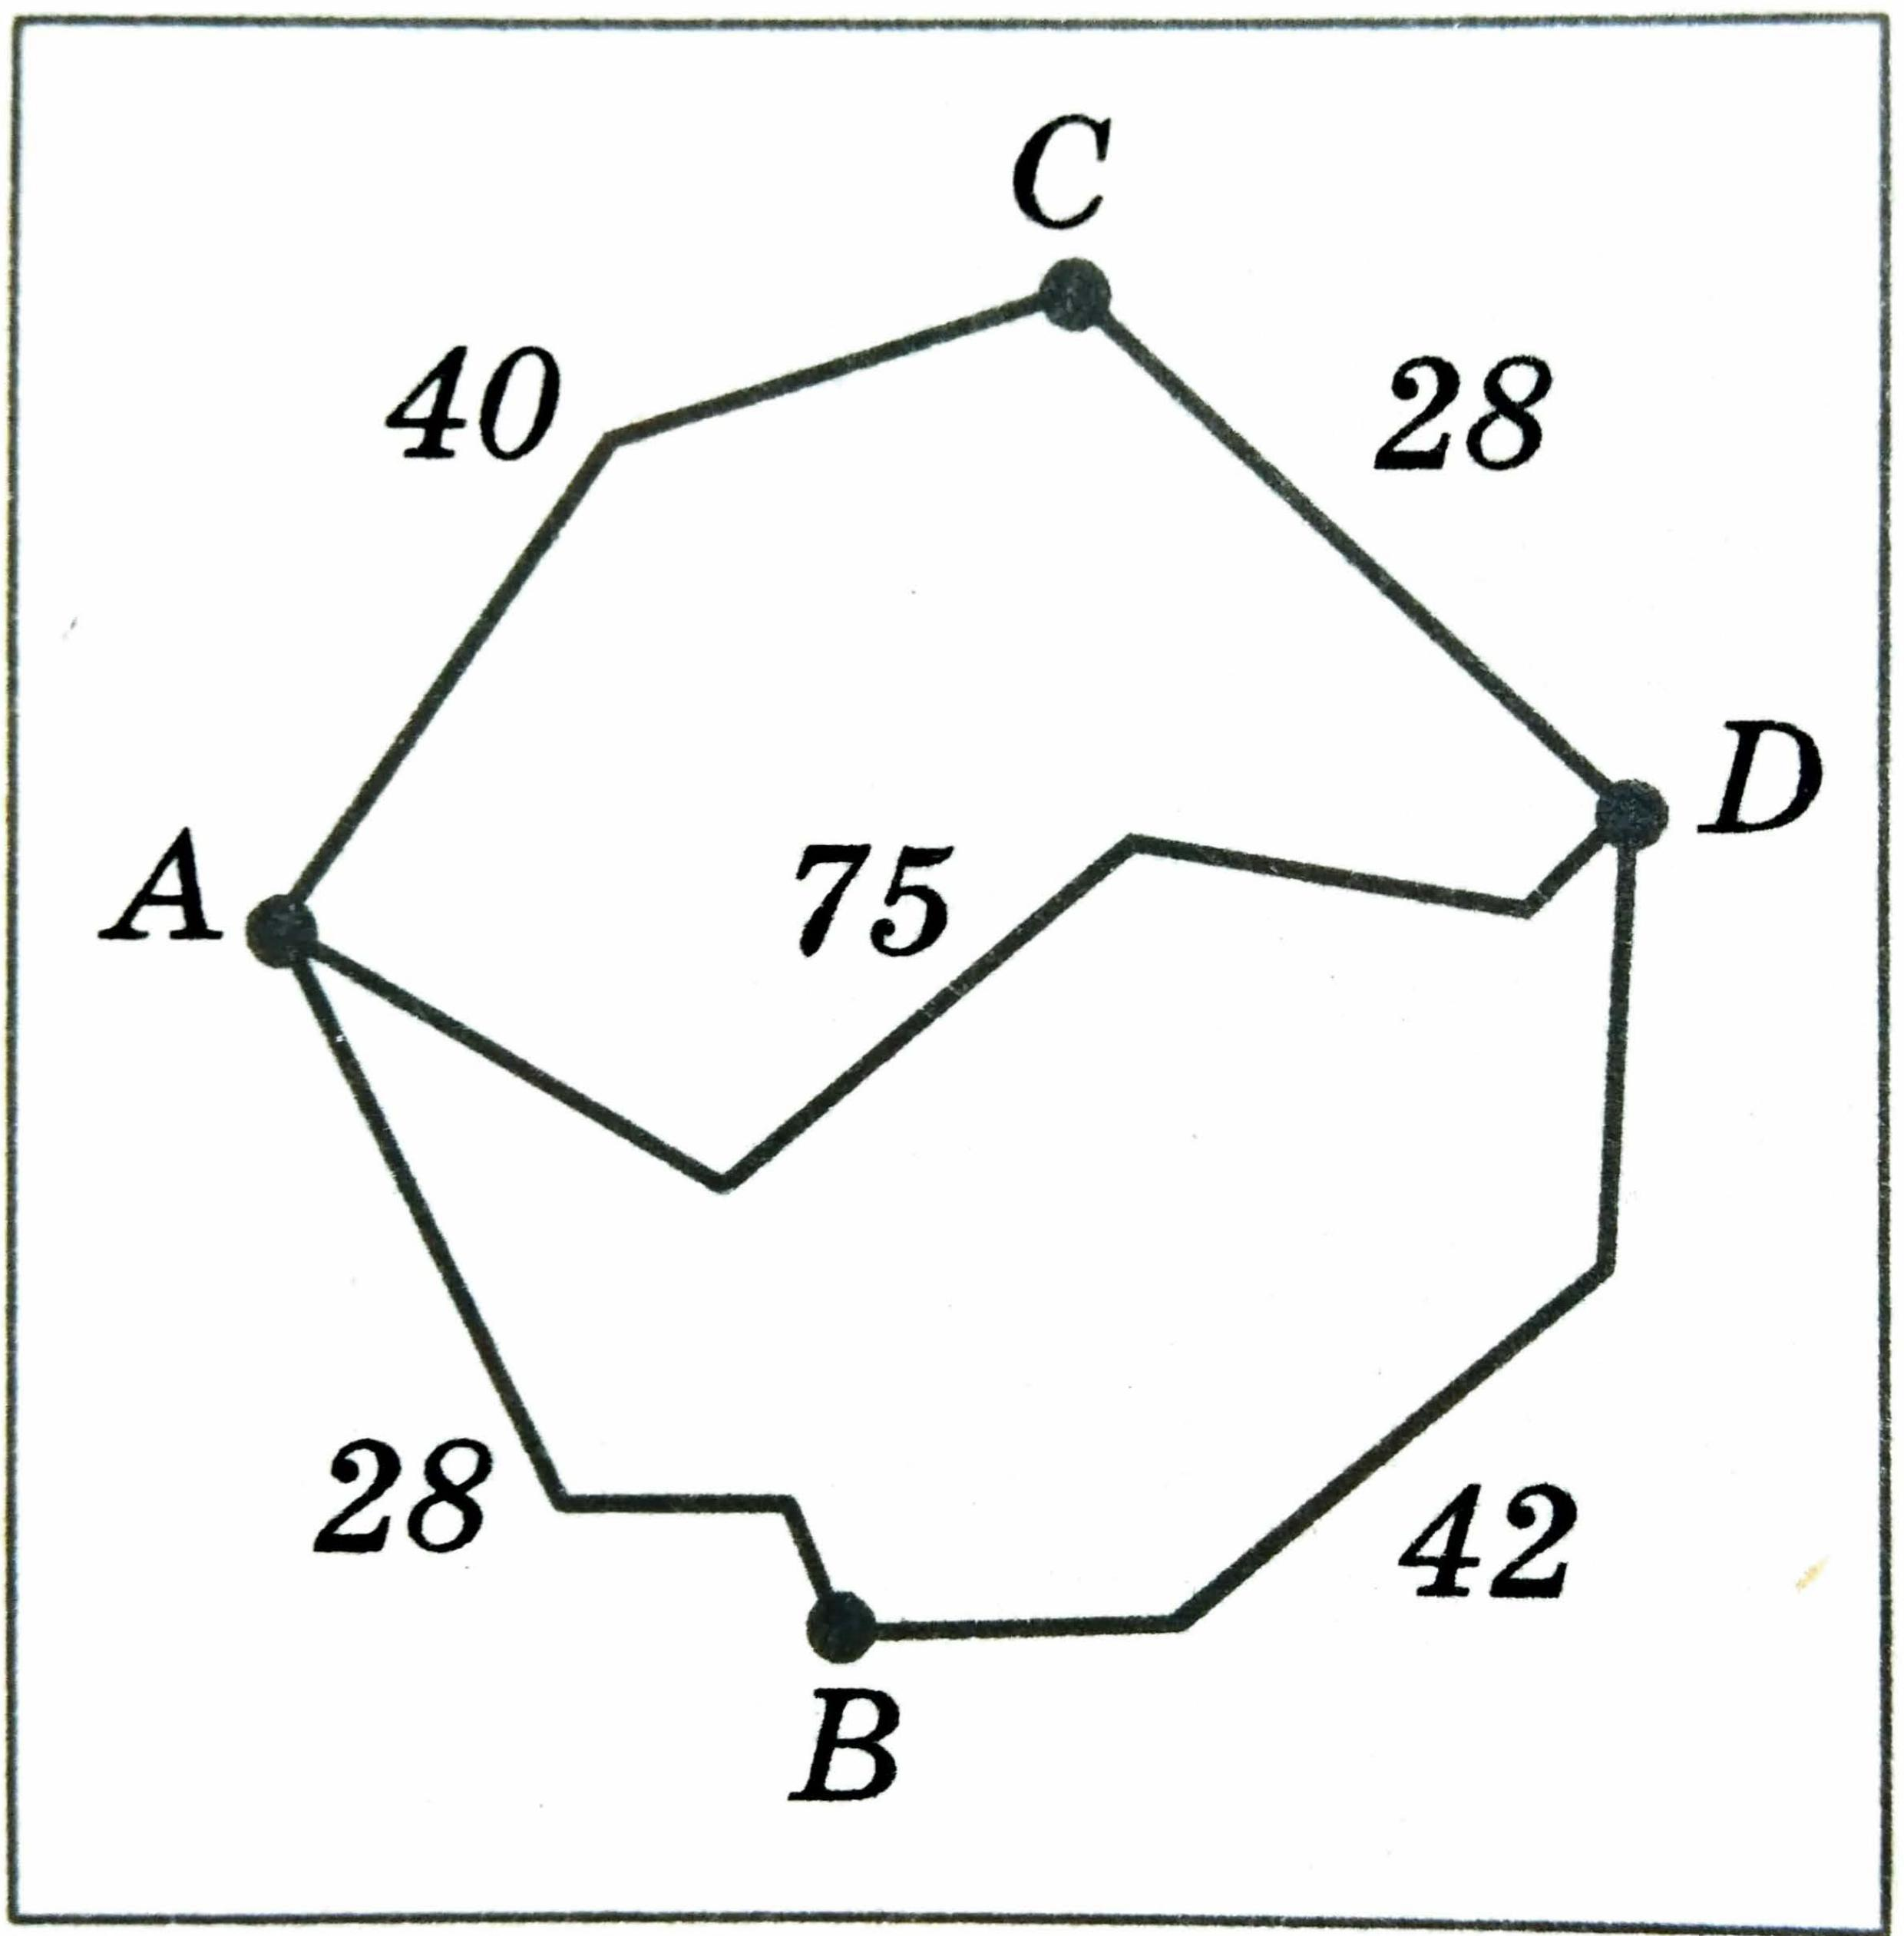
\includegraphics[width=\linewidth]{6K-16}
        \end{figure}
    \end{minipage}
\end{minipage}}
{НаписанноеРешение}
{ВерныйОтвет}{Подсказка}
\end{problem}

\begin{problem}{Сравнение, сложение и вычитание дробей.}{6.2.4}{6K}{(лёгкая)}
{Что выгоднее~--- пакет пряников весом $300$ грамм, купленный в магазине за $95$ рублей, или пряники, которые продаются на развес за $350$ рублей/кг?}
{НаписанноеРешение}
{ВерныйОтвет}{Подсказка}
\end{problem}

\begin{problem}{Сравнение, сложение и вычитание дробей.}{6.2.4}{6K}{(лёгкая)}
{Мама может почистить всю картошку за $4$ минуты, а Вовочка~--- за $12$.\\ За сколько минут они почистят её вместе?}
{Выясним, что произойдёт за одну минуту. Мама почистит в 4 раза меньше, чем всю картошку, то есть $\frac14$ от неё. Вовочка же почистит лишь $\frac{1}{12}$.\\ Тогда, поскольку они работают сообща, и вся почищенная картошка складывается, всего за минуту будет почищена $\frac{1}{4} + \frac{1}{12} = \frac{3}{12} + \frac{1}{12} = \frac{4}{12} = \frac13$ всей картошки.\\
В таком случае через три минуты ($\frac13 \cdot 3 = 1$) будет почищена вся картошка, поэтому ответ на задачу --- три минуты.}
{Мама и Вовочка вместе почистят всю картошку за 3 минуты.}{Сколько очищает каждый за одну минуту?}
\end{problem}

\begin{problem}{Сравнение, сложение и вычитание дробей.}{6.2.4}{6K}{*}
{Чтобы не заснуть, глядя на поплавки, рыбак начал рассуждать над теоретическими вопросами:
\\a) Если $3$ карася тяжелее $4$ окуней, значит ли это, что $4$ карася тяжелее $5$ окуней?
\\b) Если $4$ окуня тяжелее $3$ лещей, значит ли это, что $5$ окуней тяжелее $4$ лещей?\\
Каковы верные ответы на вопросы рыбака, если все рыбы одного вида весят одинаково?}
{а) Единственное, что нам известно~--- что 3 карася тяжелее 4 окуней. Тогда мы можем точно сказать, что 6 карасей тяжелее 8 окуней. А 15 карасей, соответственно, тяжелее 20 окуней. Можно ослабить это утверждение, и заметить, что тогда и 16 карасей тяжелее 20 окуней. Но это означает, что если взять в четыре раза меньше рыб, то 4 карася тяжелее 5 окуней! Доказано.\smallskip\\
b) Попробуем доказать то же самое в данном случае. 4 окуня тяжелее 3 лещей $\;\Rightarrow\;$ 20 окуней тяжелее 15 лещей. Но 5 окуней тяжелее 4 лещей в том и только в том случае, если 20 окуней тяжелее 16 лещей. А это из доказанного не следует: при добавлении ещё одного леща, окуни могут оказаться легче.\\ То есть точный ответ нам в данном случае неизвестен $\;\Rightarrow\;$ нет, не значит.}
{a) Да, значит. b) Нет, не значит~--- могут быть и тяжелее, и легче.}{6 карасей тяжелее 8 окуней...}
\end{problem}

\begin{problem}{Сравнение, сложение и вычитание дробей.}{6.2.4}{6S}{*}
{Бассейн наполняется двумя трубами за 48 мин, если открыть сразу обе трубы. Через одну трубу бассейн может наполниться за 2 ч. Найти объём бассейна, если известно, что за 1 мин через вторую трубу поступает на 50м$^{3}$ воды больше, чем через первую.}
{Через одну трубу за час наполняется $\frac12$ бассейна.\\ Тогда за $48$ минут $ = \frac45$ часа эта труба наполнит $\frac45$ от этого количества, а именно $\frac12\cdot\frac45 = \frac{4}{10} = \frac25$ бассейна. Значит, оставшиеся $1 - \frac25 = \frac35$ бассейна были наполнены второй трубой. Получается, что за 48 минут вторая труба наполняет на $\frac15$ бассейна больше, чем первая. Но при этом понятно, что за 48 минут через вторую трубу поступает на $48 \cdot 50 = 2400$м$^3$ воды больше, чем через первую. Значит, $2400$м$^3$ --- это $\frac15$ бассейна, а весь бассейн имеет объём в 5 раз больше: $2400 \cdot 5 = 12000$м$^3$.}
{Бассейн имеет объём $12000$м$^3$.}{Какую часть бассейна наполняет первая труба за час?\\ Какую часть часа составляют 48 минут? Какая часть бассейна была наполнена второй трубой? На сколько больше наполнила вторая труба, чем вторая?}
\end{problem}

\begin{problem}{Сложение и вычитание смешанных чисел.}{6.2.5}{6S}{(лёгкая)}
{Надо было доставить 3 бидона с молоком по $8\frac{1}{2}$ литра в каждом; для этого пришлось из одного бидона перелить $2\frac{2}{5}$ л молока в другой бидон и $1\frac{1}{4}$ л в третий. Сколько молока было первоначально в каждом из 3 бидонов?}
{НаписанноеРешение}
{ВерныйОтвет}{Подсказка}
\end{problem}

\end{document}